\chapter{Szimulációs környezet fejlesztése}
A munka fő célja a roboton futó arcfelismerő modul gyorsabbá tétele volt. Egy program futása több módon is gyorsítható. Egyik alapvető módszer lehetne erősebb hardvert alkalmazni. Ezt esetünkben két okból kiindulva elvetettem. Egyik ok, hogy a hardver adott. A robot segítségével a diplomamunkám folytatása által átölelt időszakban is aktívan kísérletsorozatot végeztek. Másik ok, hogy amennyiben esetlegesen hardveres bővítést végzünk a roboton, akkor annak két töltés közötti hasznos ideje valamilyen mértékben mindenképpen csökkenni fog. Ezeket a szempontokat és hogy a roboton jelenleg képes futni egy kezdetleges megoldás figyelembe véve a hardveres bővítések ötletét első körben elvetettem.

Amennyiben a szoftveres oldalt tekintjük szintén több lehetőségünk adódik. Egyik oldalról fejleszthetjük a futtatni kívánt programunkat, jobb algoritmusokat választva. Mivel az előzetes fejlesztések során a cél annak alapvető működőképessége volt, azt a saját leírása szerint "a világ legegyszerűbb arcfelismerő könyvtára"\cite{geitgey_face_recognition_2021} biztosítja. Ennél jobban optimalizált, illetve modernebb megoldást választva vélhetően jelentős javulás érhető el. Az ezzel kapcsolatos munkálatokat a következő fejezetben tárgyalom.

Másik lehetőségünk, hogy a roboton futó egyéb szoftvereket optimalizálva vagy az esetleges feleslegesen futó szoftvereket leállítva a saját programunk számára extra erőforrásokat szabadíthatunk fel. Ennek segítségével azon túl, hogy a feladatunk megoldására extra számítási és/vagy memóriapacitást biztosíthatunk, potenciálisan a robot általános teljesítménye is javulhat.

Mindegyik említett módszer alkalmazásához először a robot megismerése szükséges - mind hardveres, mind szoftveres téren. Nulladik lépésben emiatt a kutatott témakör irodalmi megismerése mellett ezzel foglalkoztam.

Bár az általam végzett fejlesztés szempontjából nem kritikus, mégis hasznosnak ígérkező extra lépés volt szimulációs környezetet biztosítani a robot számára. Erre elsősorban az enyémmel párhuzamosan futó navigációs fejlesztések miatt volt szükség. Emellett hasznosnak ígérkezett esetleges újabb lezárások esetén illetve egyéb, távmunkát igénylő esetekre, mint például egy külföldi hallgató becsatlakozása.

\section{A robot felépítése}
A robot alapját egy RB-1 BASE henger alakú mobil platform képzi. Átmérője 500mm. USB, Ethernet és HDMI portokkal rendelkezik. Wifi segítségével vezeték nélküli kommunikácóra is képes. 50kg súly elszállítására képes, két töltés közötti üzemideje 10 óra. A benne elhelyezett számítógép Intel i5-ös processzorral és 8 Gb memóriával rendelkezik, melyen 16-os verziószámú Ubuntu Linux rendszer fut. Az alap részletes specifikációi a
\ref{tab:rb1_base_specifications}. táblázatban találhatóak.

\begin{table}[!ht]
    \footnotesize
    \centering
    \renewcommand{\arraystretch}{1.5}
    \begin{tabular} {|r | l |}
        \hline
        Méret & 500 x 215 mm \\
        \hline
        Súly & 30kg \\
        \hline
        Teherbírás & 50kg \\
        \hline
        Sebesség & 1.5 m/s \\
        \hline
        Üzemidő (két töltés között) & 10 óra \\
        \hline
        \hline
        Processzor & Intel i5 \\
        \hline
        Memória & 8 Gb \\
        \hline
        Portok száma & 2 x USB, 1 x Ethernet, 1 x HDMI \\
        \hline
        \hline
        Operációs rendszer & Ubuntu 16 \\
        \hline
        ROS verzió & Kinetic Kame \\
        \hline
        Vezeték nélküli kommunikáció & WiFi 802.11n \\
        \hline
    \end{tabular}
    \caption{Az RB-1 base scpecifikációi.}
    \label{tab:rb1_base_specifications}
\end{table}

Biscee fejlesztése során a paltform egy felépítménnyel és több hardveres kiegészítéssel is el lett látva. A felépítmény anyaga alumínium, fő részei a robothoz rögzített oszlop és az ehhez az oszlophoz derékmagasságban csatlakozó hordtálca. A hordtálca anyaga fa. Mivel a robot wifi jelét a beépített router helyzete miatt jelentősen árnyékolja a felépítmény alatt egy kisméretű switch hub lett elhelyezve. A hordtálca kerülete mentén 7 ultrahang szenzor lett elhelyezve, ebből 6 navigációs, 1 pedig kommunikációs célt szolgál. A szenzorok értékeit Arduino mikrokontrollerek olvassák ki, az értékeket USB-n keresztül továbbítják a robot számára egy USB hubon keresztül. A robot kamerái az oszlop tetején kialakított fejrészen helyezkednek el. A fejrész mozgatását két DYNAMIXEL szervó teszi lehetővé. A kábelezés eltakarása és a természetes hatás keltésének érdekében a robotot műbőr borítással látták el. A hordtálcáról lelógó csíkozott műbőr szoknya könnyű hozzáférést biztosít a hubokhoz és a kábelezéshez. A leírtak megfigyelhetőek a
\todo{ábra}. ábrán.

\section{ROS, szimulációs és virtualizációs lehetőségek}
A roboton a Robot Operating System (ROS) Kinetic Kame verziója fut. Bár a ROS elviekben bármilyen Linux alapú rendszeren, illetve akár Windows alatt is futtatható, hivatalos kiadásai szorosan kötődnek az Ubuntu Linux operációs rendszerhez. A napjainkra már EOL (End Of Life - élete végére ért) Kinetic Kame kiadás az Ubuntu 16 (Xenial Xerus) LTS (Long Term Support - hosszú támogatási idejű) verziójához jött ki, mely mára szintén EOL rendszer. Ez szempontunkból azért különösen lényeges, mert a szimuláció fejlesztésekor a felhasznált csomagok verzióinak egyeztetése szükséges. Szerencsére mára több virtualizációs lehetőség is létezik, melyek segítségével direkt telepítés nélkül is képesek vagyunk egy bizonyos operációs rendszer futtatására. A szimuláció fejlesztése elosztott feladatként folyt. A robot felépítményéről 3D modell készült, a robot teszteléséhez használt teremről pedig gazebo világ. Ezek a \ref{fig:3d_model_and_gazebo_world}. ábrán láthatóak. A diplomamunka részfeladatának tárgyát az RB-1 Base létező szimulációjának ezekkel és a hozzáadott szenzorokkal történő kiegészítése képzi. A fejlesztési környezet az alacsony belépőszint és könnyű megoszthatóság miatt egy Oracle VM Virtualbox\cite{noauthor_oracle_nodate} virtuális gépen történt. A szimuláció továbbá tesztelten sikeresen futtatható WSL\cite{craigloewen-msft_wsl_nodate} alatt és konténerizálva Docker\cite{noauthor_docker_nodate} vagy SingularityCE\cite{noauthor_singularityce_nodate} alatt.

\begin{figure}
    \centering
    \begin{subfigure}[b]{0.45\linewidth}
        \includegraphics[height=7cm]{figures/biscee_model.png}
    \end{subfigure}
    \begin{subfigure}[b]{0.45\linewidth}
        \includegraphics[width=\linewidth]{figures/simulation_from_above.png}
    \end{subfigure}
    \caption{A szimulációhoz készült 3D modell és Gazebo world.}
    \label{fig:3d_model_and_gazebo_world}
\end{figure}

A ROS beépített fizikai szimulációra alkalmas környezetet nem tartalmaz. A legelterjedtemm megoldás erre a Gazebo robotszimulátor alkalmazása. A \lstinline{gazebo_ros_pkgs} metacsomag által rendelkezésünkre álló wrapperek segítségével könnyen hozhatunk létre és indíthatunk el ROS-on belülről robotmodelleket és szimulációkat.

A Gazebo a szimulációk leírásához SDF (Simulated Description Format) fájlokat használ, mely egy objektumok, környezetek és az ezek közötti kapcsolatok leírására specializált XML formátum. Ezzel szemben a ROS a robotok leírásához az URDF (Universal Robotic Description Format) formátumot használja. Amint neve sugallja, ez az előzővel szemben robotok leírására alkalmas. Szerencsére az ezek közötti konverzió megoldott, ezért elegendő az utóbbit létrehoznunk. Az egyszerűbb kezelhetőség érdekében lehetőségünk áll továbbá xacro makrók használatára. A leírtak és az URDF működésének szemléltetésére jó példa az eredeti robot szimulációjának kiegészítése az elkészült 3D modellel és ultrahang szenzorokkal. Az urdf tartalmának a \lstinline{<robot>} tagen belül kell elhelyezkednie. A többször használandó értékeket definiálhatjuk \lstinline{xacro:property}ként, így azokat globálisan tudjuk állítani esetleges változás vagy elírás esetén. 
\lstinputlisting[language=XML]{figures/code/urdf_xacro_basic.xml}
A robotunkat jointokból (csukló) és linkekből (tag) építjük fel. Az eredeti robot rendelkezik egy bázisként szolgáló taggal, először ehhez írunk le egy kapcsolatot egy csukló segítségével. Ehhez először meg kell adnunk ennek típusát és helyzetét. Esetünkben ez egy fix eltolást jelent a bázistól, ezért típusink "fixed" és az \lstinline{origin} tagen belül egy z irányú eltolást definiálunk. Ezt követően megadjuk a csuklót követő és az az előtti tagokat a \lstinline{child} és a \lstinline{parent} tagek segítségével.
\lstinputlisting[language=XML]{figures/code/urdf_joint.xml}
A tagok leírása kissé hosszabb, hiszen ezek képzik a robotunk fizikai elemeit. Itt kell megadnunk a részek inerciális értéket. Fontos részleg, hogy a részek számár külön definiálhatunk ütközési alakot és vizuális kinézetet. Ezek közül mindkettő \lstinline{geometry} tagek segítségével történik. Használhatunk egyszerű alakzatokat, mint téglatestek vagy hengerek. Amennyiben az adott rész alakja jól közelíthető ezek valamelyikével érdemes lehet ütközési alakzatként azt alakamaznunk. Használhatunk továbbá egyedi modelleket is a \lstinline{mesh} tag segítségével.
\lstinputlisting[language=XML]{figures/code/urdf_link.xml}
A szenzorok definíciója a \lstinline{gazebo} taggel történik. Ennek meg kel adnunk, mely tagunkhoz tartozik a szenzor. Ez után következnek a szenzorhoz tartozó tulajdonságok leírásai, egy UH szenzor esetén ez a kibocsájtott sugárzás. Meg kell adnunk továbbá a szimulációhoz szükséges gazebo plugint is. Ezen belül definiálhatjuk a szimuláció további részleteit és a szenzorok által használt ROS topicokat.
\lstinputlisting[language=XML]{figures/code/urdf_gazebo.xml}
Amennyiben megírtuk a szükséges kiegészítéseket, az ezeket tartalmazó filet xacro segítségével egyszerű beemelhetjük a robot eredeti leírásába.
\begin{lstlisting}
    <xacro:include filename="$(find rb1_base_description)/urdf/custom_stuff/custom_stuff.urdf.xacro"/>
\end{lstlisting}
Az újrahasználhatóság és az egyszerű konfiguráció érdekében saját makrókat is létrehozhatunk. Esetünkben például a bisceen használt ultrahang modulokhoz ez előnyös megoldás volt, hiszen 6 ugyan olyan szenzor is elhelyezésre került különböző pontokon. A makrók számára paraméterek adhatóak meg, melyek segítségével az adott alkalmazás pontosítható.
\begin{lstlisting}
    <xacro:macro name="sensor_biscee_ultrasound" params="prefix parent prefix_topic:='uh' *origin min_angle:=-0.14835 max_angle:=0.14835 uh_fov:=0.2967 gpu:=^|true">
\end{lstlisting}
A szenzorokat ezt követően egyszerűen hozzáadhatjuk a robot leírásához.
\begin{lstlisting}
<xacro:sensor_biscee_ultrasound prefix="$(arg prefix)front_bottom_ultrasound" parent="$(arg prefix)base_link" prefix_topic="/front_bottom_ultrasound">
    <origin xyz="0.223 0.0 1.159" rpy="0 3.1416 3.1416"/>
</xacro:sensor_biscee_ultrasound>
\end{lstlisting}
A szimuláció az \lstinline{rb1_base_sim} csomag segítségével futtatható. Megfelelően átkonfigurálva és a bisceet indító launch fileba illesztve a szimuláció egyetlen \lstinline{roslaunch} parancs futtatásával elindítható. A szimuláció során a beépített rViz\cite{noauthor_rviz_nodate} vizualizáció is fut, melynek segítségével a robot által érzékelt környezetet és útvonaltervezést ellenőrizhetjük. A szimuláció futás közben a \ref{fig:simulation_gazebo_and_rviz}.ábrán látható Szükség esetén akár saját navigációs pontot is hozzáadhatunk.

\begin{figure}
    \centering
    \includegraphics[width=\linewidth]{figures/simulation_gazebo_and_rviz.png}
    \caption{Gazebo szimuláció és rViz.}
    \label{fig:simulation_gazebo_and_rviz}
\end{figure}

Sajnos a fejlesztés során kiderült, hogy a kamerák szimulációja sem virtuális gépen, sem konténerben futtatva nem működőképes. Ennek ellenére a szimuláció fejlesztése nem csak az egyéb fejlesztésekhez, hanem számomra is hasznosnak bizonyult, mivel menet közben megismertem a nodeok konténerben futtatásának lehetőségét. Ez lehetőséget biztosít, hogy a roboton futó régi operációr rendszer ellenére újabb rendszereken elérhető megoldásokat alkalmazzunk.

\chapter{A potenciális algoritmusok kiválasztása}

A fejlesztői munka természeténél fogva iteratív. Első lépésként a roboton jelenleg futó megoldásból és internetes keresés alapján meghatároztam a potenciális algorimusokat. Ezt követően felkutattam ezek létező implementációit. Ezt felhasználva előzetesen rögzített és élő kameraképet feldolgozva először előzetes szűrést végeztem pontatlan és/vagy lassú megoldások kiszűrésére. Lévén az egyes cikkek és git repositoryk gyakran egymásra hivatkoznak vagy több algoritmust/implementációt is tartalmaznak az implementáció-tesztelés és az irodalmi kutatás egymáshoz viszonyított helyzete változó volt. Az írott forma átláthatóságát az ily módon történő tárgyalás jelentősen akadályozná, ezért a következőkben az algoritmusokat és keretrendszereket általam választott sorrendben tárgyalom. Fontos továbbá megemlíteni, hogy az egyes algoritmusok és az alkalmazott keretrendszerek/könyvtárak neurális hálózatok esetén legtöbbször egymástól függetlenek. Egy tetszőlegesen választott struktúrát implementálhatunk Caffe, Pytorch és Tensorflow segítségével is. A választás során ezért előnyben részesítettem azokat az implementációkat, melyek lehetőleg a képek kinyerésére amúgy is felhasznált OpenCV könyvtárat használják, hiszen ez emiatt előre telepítve van a roboton. ROS nodeokat implementálhatunk mind C++, mind Python nyelven. Bár C++ használatával vélhetően kismértékben gyorsabb implementációk lennének létrehozhatóak, a könyvtárak verzióinak változására tapasztalataim szerint érzékenyebb, nehezebben frissíthető kódot kapunk.

Jellemző probléma volt az egyes megoldások, de még inkább az egyes kiértékelő programok esetén a verziók egyeztetése. A Python által nyújtott virtuális környezetek és csomagkezelés rugalmas megoldást képesek nyújtani ennek kiküszöbölésére. C++ esetén a legjobb megoldásnak a szimulációnál már bevált Docker konténerek alkalmazása bizonyult.

\section{Az algorimusok előzetes értékelése}
Az összehasonlításhoz először azonosítani kell a jelölteket. Az arcdetekció extenzív irodalommal rendelkezik, így nagy létszámú jelöltből kell választanunk. Ezen lépés célja, hogy feltárja azokat a megoldásokat, amelyek potenciálisan kielégítik az adott feltételeket. Ezek közül esetünkben a legfontosabb a jelenleginél nagyobb sebesség biztosítása legalább összemérhető pontosság mellett. Fontos továbbá, hogy rendelkezésünkre álljon az algoritmus valamilyen mértékű implementációja, hiszem a magas számú jelölt miatt nem áll rendelkezésünkre az idő és a tanításhoz szükséges számíási kapacitás sem.

A ROS \lstinline{cv_bridge} csomagja segítségével rendelkezésünkre áll az OpenCV\cite{noauthor_opencvopencv_2021} könyvtárral való együttműködéshez szükséges interfész, mely a roboton előzetesen is rendelkezésre áll. Ebből kifolyólag és a széleskörű elterjedtségének köszönhetően ezt a könyvtárat választottam képfeldolgozáshoz. Segítségével könnyen olvashatunk be képeket és videókat, a számtalan beépített konverziós függvény segítségével pedig könnyen létrehozhatjuk az különböző igényelt bemeneteket. Könnyen kezelhetjük továbbá a számítógéphez csatlakoztatott webkamerákat, ami a választás során igen hasznosnak bizonyult. Élő kamerakép segítségével gyorsan és rugalmasan tesztelhetjük a talált algoritmust, előzetes képet kapva annak sebességéről és a felismerés limitációiról. A \ref{fig:selection_webcam}. ábrán látható példán például az első esetben az algoritmus sikeresen felismeri a frontális és profilnézetű arcot is, viszont a második esetben látható, hogy a jelentősen oldalra fordított frontális arcot már nem képes detektálni. Amennyiben az algoritmust több személy detektálására kívánjuk tesztelni partner vagy a képen látható módon képes segítségével is megtehetjük. Az előre elkészített képekkel szemben ez a módszer ennél a lépésnél előnyt jelent, mert a teszt az eredményektől függően könnyedén, adaptívan változtatható. Emellett az ember számára könnyen feldolgozható információt biztosít az algoritmus sebességéről is.

\begin{figure}
    \centering
    \begin{subfigure}[b]{0.45\linewidth}
        \includegraphics[width=\linewidth]{figures/selection_webcam_linus_good.png}
    \end{subfigure}
    \begin{subfigure}[b]{0.45\linewidth}
        \includegraphics[width=\linewidth]{figures/selection_webcam_linus_bad.png}
    \end{subfigure}
    \caption{Algoritmus tesztelése webkamera segítségével.}
    \label{fig:selection_webcam}
\end{figure}

\section{HAAR kaszkád (OpenCV)}
Alapja a Viola és Jones által “Rapid Object Detection using a Boosted Cascade of Simple Features”\cite{viola_rapid_2001} című cikkükben bemutatott és “Robust Real-Time Face Detection”\cite{viola_robust_2004} című cikkükben (közel) valós idejű arcdetekcióra alkalmazott algoritmus. A módszer működésének alapját az irodalmi áttekintésnél már ismertettem.

Annak ellenére, hogy két évtizedes technológiáról beszélünk, alkalmazása még ma is igen elterjedt. Régebbi vagy akár mai olcsóbb videokamerák és fényképezőgépek ezt a módszert alkalmazzák. A ROS egyetlen hivatalos arcfelismerő csomagja \cite{noauthor_face_detector_nodate} is kaszkád alapú.

Az OpenCV könyvtár beépített példái között több arcfelismerésre alkalmazható kaszkádot is találhatunk. Ezek leírását xml fájlok tartalmazzák, melyeket megtekinthetünk a hivatalos Github repositoryban\cite{noauthor_opencvopencv_2021}, a \lstinline{data/haarcascades} mappa alatt. A módszer fő hátulütőjéről előzetes sejtést adhat, hogy találhatunk \lstinline{haar_frontalface.xml} és \lstinline{haar_profileface.xml} verziókat, de egybevontat nem. A fileokat megtekintve megtudhatjuk továbbá, hogy a kaszkádok függőleges arcokat feltételeznek.

\section{HoG (Dlib)}
\todo{megírni}
A roboton jelenleg futó algoritmus. Az alap szint, melyet a jelölteknek el kell érnie.

\section{ResNet-10 SSD (OpenCV Caffe)}
A háló ötvözése a "SSD: Single Shot MultiBox Detector"\cite{liu_ssd_2016} és "Deep Residual Learning for Image Recognition"\cite{he_deep_2015} cikkekben bemutattott módszereknek. Az SSD módszer három fő alrészre bontható, melyek a
\ref{fig:ssd_multibox_detector}
ábrán láthatóak. A módszer alapját konvolúciós rétegek képzik.

\begin{figure}
    \centering
    \includegraphics[width=\linewidth]{figures/ssd_multibox_detector.png}
    \caption{SSD MultiBox detektor sematikus ábrája}
    \label{fig:ssd_multibox_detector}
\end{figure}

Első lépése a jellemzők kinyerése, mely lényegében képosztályzást jelent. Bemenete egy kép, melyre tekinthetünk egy 3 csatornás feature mapként (jellemző térkép). Kimenete jellemzően kisebb méretű, ám jóval több csatornából áll. Ezt az eredeti megoldásban egy VGG\cite{simonyan_very_2015} hálózatra alapozták. A különböző méretű detekciók végrehajtásának érdekében még a jellemzőkinyerés lépésén belül a kinyert jellemzőket további konvolúciós hálózatok piramisán küldjük keresztül, melyek egyre kisebb méretű kimenetekkel rendelkeznek. A köztes kimeneteket eltároljuk a következő lépés számára.

Második lépésben következik a detekciós fázis. A módszer fix számú alapvető predikciós dobozt feltételez, melyet jelöljünk \(n_A\)-val. Ezek a dobozok a konvolúciós viselkedésnek megfelelően csempézik ki a képet. A detektoraink generált feature mapenként minden dobozhoz két kimenetet generálnak. Az első az objektumosztályoknak megfelelő \(n_C\) darab konfidencia értéket tartalmazza. A második dobozonként 4 transzformációs értéket a doboz (x, y) pozícióját és (h, w) magassát és szélességét illetően, a detekció pontosításának érdekében.

Harmadik lépésben NMS-t (Non Maximum Supression) végzünk a többszörös detekciók kiküszöbölésének érdekében. Ennek oka, hogy a különböző méretű és alakú dobozok közül várhatóan egy-egy objektumot többön belül is érzékelni fogunk. Ennek érdekében a nagyban átfedő négyzetek közül csak a legmagasabb konfidencia értékkel rendelkezőt tartjuk meg.

\section{FaceBoxes (Pytorch)}
A "Faceboxes: A CPU real-time and accurate unconstrained face detector" című cikkben tárgyalt algoritmus két fő részre osztható, melyek megfigyelhetőek a
\ref{fig:faceboxes}. ábrán.

\begin{figure}[h]
    \centering
    \includegraphics[width=\linewidth]{figures/faceboxes_framework.jpg}
    \caption{A faceboxes algoritmus felépítése. Az ábra az eredeti cikkhez\cite{zhang_faceboxes_2018} tartozó hivatalos github repositoryból\cite{zhang_faceboxes_2021} adoptálva.}
    \label{fig:faceboxes}
\end{figure}

Az első, a Rapidly Digested Concolution Layers (RDCN, "Gyorsan Emésztett Konvolúciós Rétegek") nevet kapta. Fő észrevétele, hogy a nagy bemenet, kernelméret és kimenetből adódó, a CNN alapú megoldásokra jellemző lassúság megfelelően beállított paraméterek segítségével végrehajtott gyors dimenziócsökkentéssel kiküszöbölhető. Ez különösen nagy előnyt jelent CPU-n történő futtatáskor, mely tervezett felhasználási módunk számára elsődleges szempont. Másik fontos része ennek a lépésnek a C.ReLU \cite{shang_understanding_2016} aktivációs függvény alkalmazása, melynek lényege, hogy a kimenet negáltját hozzáfűzi az eredeti kimenethez. Ez igen olcsó művelet és kiküszöli a CNN-ekre jellemző szimmetrikus kimenetek betanulását.

A második szakasz a Multiple Scale Convolution Layers (MSCL, "Több Méretű Konvolúciós Rétegek"), mely három ötletet ötvöz. Első lépésben inception \cite{szegedy_going_2015} rétegek segítségével több méretnek megfelelő jellemző reprezentációkat generál a detekciós rétegek számára. Ezt követően a Feature Pyramid Network (FPN) \cite{lin_feature_2017} módszer által inspirálva a durvább felbontású feature mapek értékei bilineáris skálázással felskálázva, majd egy 1x1-es konvolúció segítségével a megfelelő csatornaszámra csökkentve a finomabb felbontásokhoz hozzáadódnak. A különböző rétegek dobozait ezt követően az SSD-hez \cite{liu_ssd_2016} hasonlóan osztják föl.
\todo{ide lehetne még írni a további két lépésről, ha kell}

Az algoritmus eredeti kódja szabadon elérhető a(z) \lstinline{sfzhan15/FaceBoxes} \cite{zhang_faceboxes_2021} Github repository alatt. Elérhető továbbá az előzőleg kifejtettek szempontjából kedvezőbb Pytorch alapú Python implementáció is a \lstinline{zisianv/FaceBoxes.Pytorch} \cite{wong_faceboxes_2021} repository alatt.

\section{BlazeFace (Mediapipe)}
A "BlazeFace: Sub-millisecond Neural Face Detection on Mobile GPUs"\cite{bazarevsky_blazeface_2019} cikk címéhez híven a tárgyalt algoritmus mobil GPU-val rendelkező eszközökre lett optimalizálva. Alapja(i) a MobileNetV2/V2 \cite{howard_mobilenets_2017, sandler_mobilenetv2_2019} algoritmusok, melyek egyébként az SSD-ből GPU barát formára módosított alapvető doboz rendszert alakalmaznak. Ez a \ref{fig:blazeface} látható. ábrán. Ezekhez képest nagyobb kernelméretű konvolúciós rétegeket alkalmaz, melyek GPU-n történő futtatás szempontjából előnyösek, a miénkből pedig sajnos meglehetősen hátrányosak. Ennek ellenére CPU-n is igen kedvező sebességek érhetőek el vele. Az ezekből álló BlazeBlock névre keresztelt egységek a \ref{fig:blazeface}. ábrán láthatóak.

\begin{figure}[h]
    \centering
    \begin{subfigure}[b]{0.45\linewidth}
        \includegraphics[width=\linewidth]{figures/blaze_block.png}
        \caption{BlazeBlock és dupla BlazeBlock}
    \end{subfigure}
    \begin{subfigure}[b]{0.45\linewidth}
        \includegraphics[width=\linewidth]{figures/blazeface_anchor_computation_vs_ssd.png}
        \caption{Előzetes jellemzőkinyerés tradícionális SSD (bal) esetén és a BlazeFace (jobb) esetén.}
    \end{subfigure}
    \caption{A BlazeFace által alkalmazott módosítások. Az ábra az eredeti cikkből\cite{bazarevsky_blazeface_2019} adoptálva.}
    \label{fig:blazeface}
\end{figure}

Az algoritmus kiválasztásának oka a Google MediaPipe\cite{noauthor_mediapipe_nodate} által nyújtott letisztult Python API és előre tanított modellek voltak. 

\section{RetinaFace (insightface)}
A 2019-ben megjelent "RetinaFace: Single-stage Dense Face Localisation in the Wild"\cite{deng_retinaface_2019} cikkben megjelent RetinaFace a legújabb algoritmus a tárgyaltak közül. Ennek köszönhetően az előzőekben tárgyalt módszerek jelentős részének alkalmazása megfigyelhető benne. A publikációban javasolt szerkezet a
\ref{fig:retinaface}. ábrán látható.

\begin{figure}[h]
    \centering
    \begin{subfigure}[b]{\linewidth}
        \includegraphics[width=\linewidth]{figures/retinaface_framework.png}
        \caption{Az algoritmus belső felépítése}
    \end{subfigure}
    \begin{subfigure}[b]{0.75\linewidth}
        \includegraphics[width=\linewidth]{figures/retinaface_multitaskloss.png}
        \caption{Az algoritmus kimenetei és az alkalmazot multitask loss szemléltetése}
    \end{subfigure}
    \caption{A RetinaFace algoritmus felépítése. Az ábra az eredeti cikkből\cite{deng_retinaface_2019} adoptálva.}
    \label{fig:retinaface}
\end{figure}

A módszer egy 5 szintű FPN inspirált jellemző piramist alkalmaz, melynek bemeneteit már a háló tanítását megelőzően előre betanított ResNet szakaszok biztosítják, ezeket C1-C6-al jelzik.
\todo{ábrához odaírni, hogy C1 omittálva lett róla}
Ebből ötnél a korrábbi megoldásoknál \cite{lin_feature_2017,lin_focal_2018} is használt föntről lefelé haladó és oldalirányú kapcsolatokkal. Ezek az ábrán a P2-P5 jelzésű rétegek. A piramis P6-al jelzett csúcsa egy 3x3-as, 2-es stride értékű konvolúcióval áll elő C5-ből. Mivel nem vesz részt a föntről lefelé csatolásban, ezért C6 jelzéssel is ellátták. Ezt követően az SSH\cite{najibi_ssh_2017} és PyramidBox\cite{tang_pyramidbox_2018} által inspirált, továbbá a 2018-as WIDER Face Challenge győztesének megoldása\cite{loy_wider_2019} alapján módosított kontextus modulokat alkalmaznak a piramis öt szintjére, ezzel növelve az érzékelőmezőt és a rigid kontextusmodellezési erőt.

Az algoritmus kiválasztásának oka a papír által ígért a technika jelenlegi állása szerint a legjobbak között szereplő pontosságán és sebessén túl az volt, hogy implementációi rendelkezésre állnak Pytorch\cite{biubug6_retinaface-pytorch_2021} és Tensorflow\cite{stan_btd_retinaface-tf2_2021} keretrendszerekre is. Az algoritmus eredeti implementációjából kinőtt InsightFace\cite{noauthor_insightface_nodate} projekt szabad szoftverként MIT Licensz alatt biztosít hozzáférést \cite{noauthor_insightface-github_2021} a mai napig folyamatosan fejlesztett modelljeikhez, melyekhez kényelmes Python könyvtár is tartozik. Amennyiben szükség és lehetőség lenen rá, a könyvtár az előre betanított algoritmusokon túl továbbtanítási lehetőséget is ad. Emellett az arcdetekción túl state-of-the art arcfelismerési algoritmusokat is rendelkezésünkre bocsájt, melyek szintén egyszerűen tovább taníthatóak. A projektre napjainkban még nem kifejezetten könnyű rátalálni, azonban a jövőben számos kis fejlesztői csapat és open source projekt létrejöttét segítheti.

\chapter{A kiválasztott algoritmusok értékelése}
A webkamerás tesztelés betekintést enged az egyes módszerek erősségeibe és hátrányaiba, azonban két jelentős limitációval is rendelkezik. Egyrészt az eredmények nem számszerűsíthetőek, ezért hasonló teljesítményű megoldások közötti választáskor nem tudunk objektív döntést hozni. Másfelől a robot kamerái a webkameraképtől több területen jelentősen különbözhetnek, mint például annak felbontása és színösszetétele. Emellett a robot feladatának teljesítése közben mozgásban van, így például a képek megvilágítása is folyamatosan változhat.

\section{Benchmark alapú összehasonlítás}
Az algoritmusok objektív összehasonlításához teszteket végeztem a korábban ismertetett benchmarkokon. A fellelhető implementációk gyakran jelentős eltérést mutatnak a publikációkban tálalt eredményekhez képest. Ennek egyik vélhető oka, hogy a gépi tanítási folyamatok sok finomhangolást igényelnek az optimális eredmények eléréséhez. A tanítási folyamat más megoldásoktól eltérő pontjai legtöbbször szerepelnek a cikkekben, az ilyen részletek azonban sokszor kihagyásra kerülnek. Emellett a véletlen inicializációnak köszönhetően akár ugyan olyan paraméterek mellett, ugyan azon a gépen futtatva a tanítást két különböző időpontban különböző eredményeket kaphatunk. Másik tényező a különböző keretrendszerek jelenléte. Az implementációt megvalósító programozó tudásától és az alkalmazott segédeszközöktől függően különbségek tapasztalhatóak azok átláthatóságában, pontosságában és sebességében.

\paragraph{ROC}\hfill

Az arcdetekció bináris klasszifikációs feladat, melyhez jellemzően két kiértékelési módszert alkalmaznak. Az első a Receiver Operating Characteristic (ROC) görbe. Ennek x tengelyén a hamis pozitívak rátája, más néven 1 - specificitás található. Ez nevéből sejthetően azt adja meg, milyen gyakran osztályzunk hibásan pozitívként egy egyébként negatív példát, melyet a következőképp számolhatunk:

\begin{equation}
    HPR = 1 - specificitás = \frac{HP}{HP + IN}
\end{equation},
ahol
\begin{itemize}
    \item HP a hamis pozitívok száma
    \item IN az igaz negatívok száma
\end{itemize}

Az y tengely értékeit az igaz pozitívok rátája, más néven a szenzitivitás adja. Ez azt számszerűzíti, milyen arányban ismerünk fel egy pozitív esetet valóban pozitívként. A következő módon számolhatjuk:

\begin{equation}
    IPR = szenzitivitás = \frac{IP}{IP + HN}
\end{equation},
ahol
\begin{itemize}
    \item IP az igaz pozitívok száma
    \item HN a hamis negatívok száma
\end{itemize}
A görbe egy pontját ezekből úgy kaphatjuk, hogy az összes predikciónkból valamilyen konfidenciaszint szerint kiválasztott halmazra kiszámoljuk és ábrázoljuk őket. Ez után a konfidenciaszintet variálva kiszámolhatjuk a többi pontot is. A klasszifikátorok pontozása a görbe alatti terület értékével történik, a nagyobb érték jobb. A módszer szemléltetése a \ref{fig:roc}. ábrán látható. A valós megoldások többnyire a véletlen találgatás (AUC = 0.5) és a tökéletes klasszifikátor (AUC = 1) között helyezkednek el, de létezhet 0.5 alatti pontszám is.

\begin{figure}
    \centering
    \begin{subfigure}[b]{0.45\linewidth}
        \includegraphics[width=\linewidth]{figures/ROC.png}
        \label{fig:roc}
    \end{subfigure}
    \begin{subfigure}[b]{0.45\linewidth}
        \includegraphics[width=\linewidth]{figures/PR.png}
        \label{fig:pr}
    \end{subfigure}
    \caption{ROC(bal) és PR(jobb) görbék.}
    \label{fig:roc_and_pr_curves}
\end{figure}

\paragraph{Precision - Recall}\hfill
A másik gyakran alkalmazott módszer a Precision - Recall görbe. Ennek tengelyei a nevében található értékek, melyeket az előzőekben használt jelölésekkel a következő módon kaphatunk meg:
\begin{equation}
    precision = PPE = \frac{IP}{IP + HP}
\end{equation}
\begin{equation}
    recall = szenzitivitás =  \frac{IP}{IP + HN}
\end{equation}
Amint látható a recall egyenlő a ROC görbénél alkalmazott szenzitivitással. A precíziót nevezhetjük még Pozitív Predikciós Értéknek (PPE) is. Értelmezése az, hogy a pozitív predikcióink mekkora részben tartalmaznak valóban pozitív eseteket. A gráf egyes pontjait a ROC-hoz hasonlóan kaphatjuk. Pontozása szintén megfeleltethető a görbe alatti területnek. Ezt legtöbbször az Átlagos Precízió (AP) számításával érik el úgy, hogy az egyes konfidenciaszintek precision értékét súlyozottan átlagolják.

\section{Összehasonlítás a robotról származó felvételeken}
A benchmark alapú összehasonlítás jó és számszerűsíthető értékelést ad az algoritmusok pontosságáról, azonban nem biztosít átfogó képet azok előnyeiről és hátrányairól specifikus felhasználási esetekben. Ez alól valamelyest kivételt képez a WIDER face adatszett, amely események szerint szeparálva tartalmaz képeket, azonban ez is csak korlátozott mértékű specificitás nyújtására alkalmas. Ennek kiküszöbölésére elemzést végeztem a robotról származó felvétel segítségével is. A felvétel egy, a robottal végzett felmérés alatt készült. Ennek köszönhetően szerepel rajta azon esetek jelentős része, amelyben a robot a valóságban emberekkel találkozhat. Emellett további előnye még az egyéb képekkel és videókkal szemben, hogy amennyiben nem történik szenzorváltás színösszetétele egyezik azzal, amelyet később éles helyzetben fel kell dolgoznunk. A mérés első lépése volt az érdekes kulcspontok azonosítása a felvételen. Ez a lépés azért volt szükséges, mert a kísérlet során a robot több alkalommal is "üresjáratban" állt, ami alatt a kép nem tartalmaz arcokat és lényegében nem is változik. A kiválasztott részleteken szerepelnek olyan klasszifikációs szempontból nehéznek minősülő, de szempontunkból lényegesnek tekinthető esetek, mint például
\begin{itemize}
    \item oldalnézetű (profil) arc
    \item hátulsó oldalnézetű arc (például mikor egy asztal felé tartunk)
    \item lefelé tekintő arc (például a menü olvasásakor)
    \item hosszú hajjal kitakart arc
    \item maszkkal kitakart arc
    \item erős háttérvilágitás miatt részben kimosódott kép (ablakkal szemben)
    \item gyenge megvilágítású arc
    \item arcot nem de tárgyakat és színes képeket tartalmazó részletek
\end{itemize}
Ezekre látható néhány példa a \ref{fig:video_examples}. ábrán. Az eddig leírt videófelvétel a kiválasztott részletekre korlátozva is több ezer képkockát tartalmaz, felbontása a standard 640x480 képpontos VGA felbontás. Ez a kamera által nyújtott 1280x1024-es nyers képektől eltér mind arányaiban, mind méretében.

Ennek kiküszöbölésére mérést végeztem a robotról származó nyers felvételen is, majd annak átméretezett verzióin. Az algoritmusok feldolgozási sebességét az esetleges szükséges bemeneti konverziókkal együtt, azonban az eredmények kiértékelése nélkül mértem le. A méréshez a Python beépített \lstinline{time} könyvtárát használtam.

\begin{figure}
    \centering
    \begin{subfigure}[b]{0.45\linewidth}
        \includegraphics[width=\linewidth]{figures/video_examples/video_example_door.png}
    \end{subfigure}
    \begin{subfigure}[b]{0.45\linewidth}
        \includegraphics[width=\linewidth]{figures/video_examples/video_example_table_1.png}
    \end{subfigure}
    \begin{subfigure}[b]{0.45\linewidth}
        \includegraphics[width=\linewidth]{figures/video_examples/video_example_table_2.png}
    \end{subfigure}
    \begin{subfigure}[b]{0.45\linewidth}
        \includegraphics[width=\linewidth]{figures/video_examples/video_example_mask.png}
    \end{subfigure}
    \begin{subfigure}[b]{0.45\linewidth}
        \includegraphics[width=\linewidth]{figures/video_examples/video_example_back_illumination.png}
    \end{subfigure}
    \begin{subfigure}[b]{0.45\linewidth}
        \includegraphics[width=\linewidth]{figures/video_examples/video_example_empty.png}
    \end{subfigure}
    \caption{Példák érdekes esetekre.}
    \label{fig:video_examples}
\end{figure}

\section{Az értékelések eredményei, a választott algoritmus}
A kiértékelést először a kisebb méretű adatszetteken hajtottam végre. Az eredmények a \ref{fig:afw_evaluation}-\ref{fig:fddb_evaluation}. ábrákon láthatóak. A kiértékelést ezeken a faceboxes készítői által ajánlott kiértékelő kóddal végeztem. A kódot tartalmazó repository a készítők által mért korábbi eredményeket is tartalmazza, ezek közül párat megtartottam összehasonlításképp. Ezek alapján megállapítható, hogy a régebbi modellek pontossága jelentősen elmarad az újakéval szemben. A faceboxes és az insightface által nyújtott modellek eredményei azonban mind olyan magasak, és közel helyezkednek el, hogy ezek alapján nem hozható releváns döntés.
\begin{figure}
    \centering
    \includegraphics[width=\linewidth]{figures/afw.png}
    \caption{AFW}
    \label{fig:afw_evaluation}
\end{figure}
\begin{figure}
    \centering
    \includegraphics[width=\linewidth]{figures/pascal.png}
    \caption{PASCAL face}
    \label{fig:pascal_evaluation}
\end{figure}
\begin{figure}
    \centering
    \includegraphics[width=\linewidth]{figures/fddb.png}
    \caption{FDDB}
    \label{fig:fddb_evaluation}
\end{figure}

A legjobb értékeket elért algoritmusokat ezért a WIDER adatszett validációs részén is teszteltem, melyhez hivatalos kiértékelő MATLAB kód tartozik. Érdekes eredmény, hogy míg a korábbi esetekben a faceboxes minden alkalommal a buffalo\_m modellhez hasonló eredményeket produkált, itt az összes insightface modellhez képest jelentősen rosszabb pontszámot ért el. Ez alapján kijelenthető, hogy amennyiben bármelyik buffalo modell gyorsabbnak bizonyul, érdemes lehet azt előnyben részesíteni, főleg mivel azokhoz API is társul, míg a faceboxes implementáció kezelése lényegesen körülményesebb.

\begin{figure}
    \centering
    \begin{subfigure}[b]{0.75\linewidth}
        \includegraphics[width=\linewidth]{figures/wider_easy.png}
        \caption{Easy}
    \end{subfigure}
    \begin{subfigure}[b]{0.75\linewidth}
        \includegraphics[width=\linewidth]{figures/wider_medium.png}
        \caption{Medium}
    \end{subfigure}
    \begin{subfigure}[b]{0.75\linewidth}
        \includegraphics[width=\linewidth]{figures/wider_hard.png}
        \caption{Hard}
    \end{subfigure}
    \caption{A WIDER adatszetten mért eredmények.}
    \label{fig:wider_evaluation}
\end{figure}

\section{ROS node kialakítása}